\documentclass{article}

\usepackage{style}
\usepackage{hyperref}


\usepackage{Sweave}
\begin{document}

\Sconcordance{concordance:gsk_malaria_vaccine_cost_one_pager.tex:gsk_malaria_vaccine_cost_one_pager.Rnw:%
1 6 1 1 0 123 1}


\vspace{20mm}


\begin{Large}
\begin{center}
Concept note
\end{center}
\end{Large}


\begin{Large}
\begin{center}
\textbf{Scaling-up malaria vaccination: an estimation of widespread implementation costs} 
\end{center}
\end{Large}


\vspace{5mm}

\begin{changemargin}{2.5cm}{2.5cm} 
\begin{center}
\begin{large}
Elisa Sicuri \hfill \emph{elisa.sicuri@isglobal.org} \\ 
Joe Brew \hfill \emph{joe.brew@isglobal.org} \\
\end{large}
\end{center}
\end{changemargin}


\vspace{6mm}

\begin{center}
\begin{large}
Institut de Salut Global de Barcelona 
\end{large}
\end{center}


\begin{changemargin}{3cm}{3cm} 

\begin{center}
\textbf{Summary}
\end{center}

\emph{As the global health community prepares for the roll-out and expansion of an effective malaria vaccine, public health authorities will need to ready the funding and logistical mechanisms to make the delivery and administration of the vaccine feasible and efficient. This "concept note" describes a proposed meta-analysis of the existing literature on the implementation costs of vaccination implementation programs in developing countries, with the aim of estimating country-specific malaria vaccine administration costs.}
\end{changemargin}
\vfill  

\newpage

\section*{Overview}

We propose to estimate the cost of implementation of widespread vaccination programs. We will generate estimates both globally and at the country-level, thereby informing and preparing the public health and scientific communities for the roll-out of widespread vaccination programs, with a special section on the potential implementation costs of a widespread malaria vaccine.


\section*{Process}

We propose a research project divided into three phases:
% \vspace{-3mm}

\begin{enumerate}
  \setlength\itemsep{0em}
\item A literature review phase, aimed at identifying, describing and synthesizing all existing knowledge pertaining to the cost of implementing\footnote{For the purposes of this project, "implementation" refers to all costs other than the purchase of the vaccine itself: procurement, transporation, storage, administration, loss, disposal, documentation, etc.} vaccination programs in malaria-endemic regions.
\item An analysis phase, in which the studies retrieved in the literature review are quantified in a standardized fashion, and compared at the country-level. The analysis phase will also consist of the generation of a statistical model to estimate the main determinants/predictors of implementation costs for the existing literature through the use of meta-analysis and regression techniques.
\item An extrapolation and dissemination phase, consisting of the estimation (for all malaria-endemic countries) of implementation costs per vaccine administered.
\end{enumerate}

\section*{Costs}

Phase 1 of this project can be carried out with minimal or no funding. Phases 2 and 3 will require funding:

\begin{itemize}
  \setlength\itemsep{0em}
\item Phase 2 will require funding for researcher time and statistical consulting (70\% of total project cost)
\item Phase 3 will require funding for researcher time, production of visualizations, and server/hosting for public-facing toolkit (20\% of total project cost)
\end{itemize}

Additionally, approximately 10\% of project cost should be allotted for writing.

\section*{Impact}

A literature review and accompanying meta-analysis of implementation costs will be impactful in both the scientific and public health communities. From a scientific point-of-view, this study will develop and detail a methodology for the standardization of complex costing data across time, and space, accounting for the intricacies of each vaccine campaign, and synthesizing knowledge so as to be relevant to future malaria vaccination campaigns. From a public health perspective, this study's results will help public health agencies prepare for the financial aspects of malaria eliminiation and eradication campaigns, as well as identify areas of high cost (so as to begin addressing those \emph{prior} to campaign implementation). 

\newpage

\section*{Knowledge products}

This project will produce not only a literature review and meta-analysis suitable for publication, but also a public-facing toolkit\footnote{Similar in form to \href{https://joebrew.shinyapps.io/ilied/}{https://joebrew.shinyapps.io/ilied/}} with visualizations and tools for use by public health authorities, such as country-specific cost estimates (below map) and costs attributable to different areas (below table). 


\begin{center}
Example knowledge product 1: country-specific implementation cost estimates
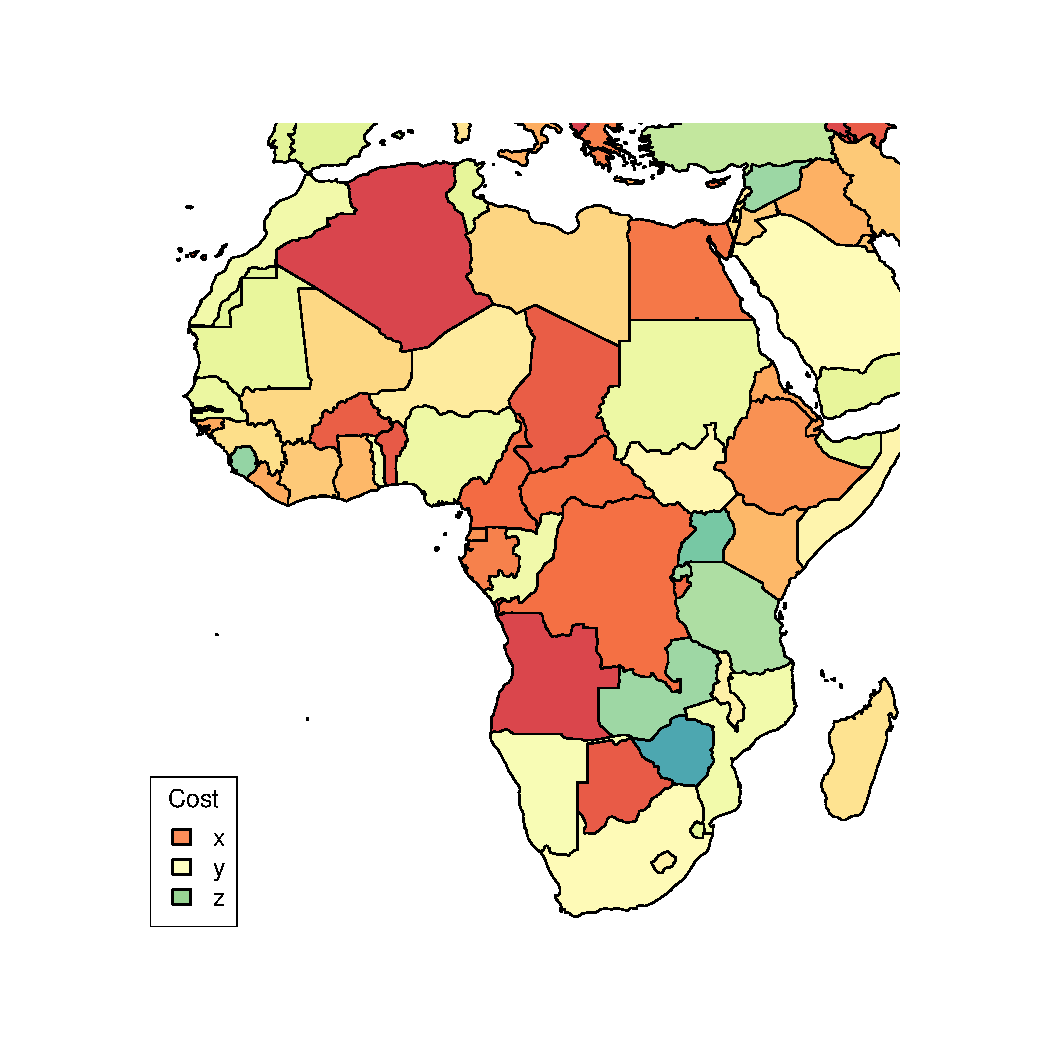
\includegraphics[width=0.5\textwidth]{map.pdf}
\end{center}

% latex table generated in R 3.2.3 by xtable 1.8-2 package
% Tue Apr 19 13:47:50 2016
\begin{center}
Example knowledge product 2: Breakdown of cost estimates by expenditure area
\end{center}
\begin{table}[ht]
\centering
\begin{tabular}{rlrrrrrr}
  \hline
 & Country & Transporation & Storage & Loss & Disposal & Documentation & Administration \\ 
  \hline
1 & Uganda & 1.14 & 0.14 & 0.11 & 0.34 & 0.15 & 1.41 \\ 
  2 & Kenya & 0.86 & 0.19 & 0.31 & 0.32 & 0.26 & 0.98 \\ 
  3 & Mozambique & 3.51 & 0.19 & 0.24 & 0.32 & 0.88 & 1.61 \\ 
   \hline
\end{tabular}
\end{table}


\vfill

% \bibliography{library}{}
% \bibliographystyle{apalike}  

\end{document}
